
Soit $\Sigma = \{R_1, \dots R_n\}$ un alphabet de symboles de relations, avec
leurs arités $a_1, \dots a_n\in\N$.

L'objectif est de créer une catégorie $\C_\Sigma$, que l'on notera $\C$ en l'absence
d'ambiguïté sur $\Sigma$, telle que la donnée d'un problème CSP soit exactement la donnée
d'un faisseau sur $\C$ (à valeur dans $\fset$, puisqu'on se limite à ce cadre là). Pour
pouvoir parler de faisceau, il faudra munir $\C$ d'une structure de site.

\subsection{Intuition}

Qu'est-ce qu'un CSP
sur un alphabet de relation $\Sigma$~? C'est la donnée d'un domaine fini $D$ et
de relations sur $D$ de bonne arité pour chaque relation de $\Sigma$. Si
$\Sigma = \{R_1, \dots R_n\}$, on peut poser la catégorie qui a pour objets
$\{\star, R_1, \dots R_n\}$ et commes flèches les identités, ainsi pour pour
tout $1\leq i\leq n$, autant de flèche de $\star$ vers $R_i$ que l'arité de
$R_i$. Un préfaisceau sur cette catégorie nous donne alors un CSP (et
vice-versa, par contre plusieurs préfaisceaux peuvent correspondre au même
CSP).

Pourquoi ne pas se contenter de ça ? Parce que cette catégorie n'est pas
intéressante pour travailler sur les CSP. En effet, elle ne contient comme
information que la liste des relations et leur arité, et rien d'autre. Nous la
noterons d'ailleurs $\Sigma$, puisque la donnée d'un alphabet de relation est
aussi exactement la donnée de leur liste et leurs arités. $\Sigma$ a donc la forme~:

\[\begin{tikzcd}
    & \star \arrow[ddl, shift right, swap, "f_1^1"]
            \arrow[ddl]
            \arrow[ddl, shift left, "f_{\text{ar}(R_1)}^1"]
            \arrow[ddr, shift right, swap, "f_1^m"]
            \arrow[ddr]
            \arrow[ddr, shift left, "f_{\text{ar}(R_m)}^m"]
            \\
    & & \\
    R_1 & \dots & R_m \\
\end{tikzcd}\]

C'est là que le résultat suivant entre en jeu.

\begin{prop}\label{canEq}
    Soit $Y : \psh(\C)\rightarrow\shc(\psh(\C))$ le plongement de Yoneda sur
    $\psh(\C)$.

    Notons $y : \C\rightarrow\psh(\C)$ le plongement de Yoneda sur $\C$. Posons~:

    \[L = \left\{\begin{array}{ccc}
             \shc(\psh(\C)) & \rightarrow & \psh(\C) \\
             F              & \mapsto     & F\circ y^\text{op} \\
    \end{array}\right.\]

    Alors $L\circ Y\cong\text{Id}_{\psh(\C)}$ et
    $Y\circ L\cong\text{Id}_{\shc(\psh(\C))}$. Cela fait de $Y$ une équivalence de
    catégories.
\end{prop}

\begin{pv}
    %TODO référence
\end{pv}

Par cet isomorphisme, $\shc(\psh(\Sigma))$ correspond aux CSP. On aimerait donc pouvoir
interpréter cette fois un préfaisceau sur $\Sigma$ comme une formule. C'est en fait assez
simple, on procède par analogie avec la façon de représenter un graphe dirigé. Un graphe
(au sens informatique) est un préfaisceau (fini) sur la catégorie $G$ suivante~:

\[\begin{tikzcd}
    v \arrow[r, bend right, "s"] \arrow[r, bend left, "t"] & e \\
\end{tikzcd}\]

Un tel préfaisceau $F : G^{\text{op}}\rightarrow\fset$ représente le graphe ayant pour
ensemble sous jacent $Fe$ et pour arrêtes $Fv$. De plus, la source d'une arrête $a\in Fv$
est $Fs(a)$ et sa destination est $Ft(a)$. On peut aussi interpréter un graphe comme
étant une formule conjonctive, dont les variables sont les points et qui possède un
unique prédicat binaire qui marque les arrêtes. On remarque que la catégorie $G$ est
exactement celle d'un alphabet avec un seul prédicat binaire. On peut donc généraliser
l'interprétation.

\begin{defi}{Formule associée à un faisceau}
    Soit $A\in\psh(\Sigma)$. On note $\phi_A$ la formule suivante~:
    
    \[\bigwedge_{1\leq i\leq m} \bigwedge_{x\in AR_i}
            R_i(Af_1^i(x), \dots Af_{\ar(R_i)}^i(x)) \]

    Avec la règle qu'une conjonction vide est $\top$

    C'est une formule conjonctive sur $\Sigma$ et dont les variables sont prises dans
    l'ensemble $A\star$.
\end{defi}

On pose alors $\C_\Sigma = \psh(\Sigma)$ notre nouvelle catégorie des formules.

\subsection{Propriétés générales de $\C_\Sigma$}

\begin{lem}
    $\C_\Sigma$ possède toutes ses limites et colimites finies.
\end{lem}

\begin{pv}
    C'est une propriété générale des catégories des faisceaux.
\end{pv}

On peut alors étudier quelques limites particulières.

\begin{lem}
    Soit $\mathbf{0}$ l'objet inital de $\C_\Sigma$. Alors $\phi_\mathbf{0}\iff\top$.
\end{lem}

\begin{pv}
    Une limite sur une catégorie de faisceau se calcule point par point. Donc $\mathbb{0}$
    est le préfaisceau qui envoie tous les objets de $\Sigma$ sur $\emptyset$ et toutes
    les flèches sur $\id_\emptyset$.

    Alors $\phi_\mathbf{0} = \bigwedge_{1\leq i\leq m}\top \iff \top$.
\end{pv}

\begin{lem}
    Soit $\mathbf{1}$ l'objet final de $\C_\Sigma$. Alors~:

    \[\phi_\mathbf{1} \iff \bigwedge_{1\leq i\leq m}R_i(x,\dots x)\]
\end{lem}

\begin{pv}
    Même démarche que pour la proposition précédente.
\end{pv}

\begin{lem}
    Soient $A$ et $B$ deux objets de $\C_\Sigma$. On note $A\wedge B$ leur coproduit
    dans $\C_\Sigma$. On a alors~:

    \[\phi_{A\wedge B} \iff \phi_A\wedge\phi_B \]
\end{lem}

\subsection{Description syntaxique des morphismes de formules}

Étudions maintenant les morphismes de formules, qui sont ici des transformations
naturelles entre faisceau. Regardons un peu plus précisément comment elles se
comportent. Soient $F,G\in\C_\psh(\Sigma)$ deux formules et $\theta:F\rightarrow F$
une transformation naturelle. Regardons comment elle doit se comporter~:

\[ \theta_\star : F\star \rightarrow G\star \]

L'existence de cette fonction nous dit que l'on renomme les variables de $F$ en des
variables de $G$, éventuellement en en contractant certaines. De plus, pour chaque
$R$ relation on a~:

\[ \theta_R : FR\rightarrow GR\]

Si on regarde comment $\phi_F$ et $\phi_G$ sont définies, cela signifie que chaque
instance de relation de $F$ est envoyée sur une instance de la même relation de $G$,
de nouveau en en contractant éventuellement certaines. Finalement, la contrainte
de naturalité est la suivante~:

\[\begin{tikzcd}
    F\star \arrow[d, "\theta_\star"] & FR_j \arrow[l, "Ff_i^j"]
                                            \arrow[d, "\theta_{R_j}"] \\
    G\star & GR_j \arrow[l, "Gf_i^j"] \\
\end{tikzcd}\]

Cela nous dit qu'après avoir renommé les variables de $F$ par $\theta_\star$, les
instance de relation sont envoyées sur des instances identiques dans $G$.

Ces différentes opérations nous rappellent un peu le calcul des séquent, et
c'est en effet le cas. Afin de le définir plus formellement, il va falloir décrire
les formules sous forme de séquents.

\begin{defi}{Séquent associé à une formule}
    Soit $\phi$ une formule conjonctive que l'on suppose mise sous la
    forme canonique $\exists x_1,\dots\exists x_n, R(\dots)\wedge R(\dots)$. On
    y associe le séquent $<\phi> = x_1,\dots x_n\vdash R(\dots), \dots, R(\dots)$.
\end{defi}

\begin{rem}
    L'habitué remarquera que la partie droite du séquent est utilisée de manière non
    canonique. En effet, elle sert usuellement à représenter une disjonction et
    l'on s'en sert ici pour représenter un conjonction. C'est lié au fait que
    les faisceaux partent de $\C_\Sigma^\text{op}$, et donc que le sens de lecture
    des règles de déduction est inversé lorsque pris par le faisceau. Ainsi, si l'on
    veut avoir des règles correspondant aux conjonctions à l'arrivée, il faut dualiser
    les règles, et cela nous donne les règles de disjonction, ce qui est cohérent avec
    l'interprétation standard des séquents.
\end{rem}

Nous rappelons maintenant les règles de déduction structurelle adaptées à nos séquents
(ce sont presque exactement celles du calcul des séquents intuitionistes).

\begin{defi}{Règles de déduction}
    Commençons par la règle de l'$\alpha$-renommage~:

    \[ \tproof{ \hypo{\Gamma, x\vdash \Delta}
         \infer1[$y\not\in\Gamma$]{\Gamma, y\vdash \Delta[x/y]} }\]

    Viennent ensuite les règles de commutation~:

    \[ \tproof{ \hypo{\Gamma, x, y, \Xi\vdash \Delta}
         \infer1{\Gamma, y, x, \Xi\vdash \Delta} }
       \qquad
       \tproof{ \hypo{\Gamma\vdash \Delta_1, R(\mathbf{x}), S(\mathbf{y}), \Delta_2}
         \infer1{\Gamma\vdash \Delta_1, S(\mathbf{y}), R(\mathbf{x}), \Delta_2} }
    \]

    Maintenant, les règles d'affaiblissement~:

    \[ \tproof{ \hypo{\Gamma\vdash\Delta}
         \infer1{\Gamma, x\vdash \Delta} }
       \qquad
       \tproof{ \hypo{\Gamma\vdash\Delta}
         \infer1{\Gamma\vdash\Delta,R(\mathbf{x})} }\]

    Enfin, les règles de contraction~:

    \[ \tproof{ \hypo{\Gamma,x,y\vdash\Delta}
         \infer1{\Gamma, x\vdash\Delta[y/x]} }
       \qquad
       \tproof{ \hypo{\Gamma\vdash\Delta, R(\mathbf{x}), R(\mathbf{x})}
         \infer1{\Gamma\vdash\Delta, R(\mathbf{x})} }\]

\end{defi}

On arrive maintenant au théorème de description syntaxique~:

\begin{theo}{Description syntaxique d'un morphisme de formule}
    Soient $F,G\in\C_\Sigma$ deux formules. Alors il existe une transformation
    naturelle $\theta:F\rightarrow G$ si et seulement si $<\phi_F>$ peut être réécrit
    en $<\phi_G>$ selon les règles de déduction ci-dessus.
\end{theo}

\begin{pv}
    Admis
\end{pv}

\begin{rem}
    On pourrait même tenter d'établir une bijection entre des arbres de preuve
    et des transformations naturelles, mais certains arbres donnent les même
    transformations, donc il faudrait quotienter par la bonne relation, ce qui
    n'est pas trivial.
\end{rem}

On peut maintenant se demander ce que donnent les constructions classiquent en terme
de séquent.

\begin{lem}\label{seqStandarts}
    Soient $\phi_1$, $\phi_2$ deux formules telles que $<\phi_1> = \Gamma\vdash\Delta$ et
    $<\phi_2> = \Xi\vdash\Omega$ (on suppose $\Gamma\cap\Xi=\emptyset$), alors~:

    \begin{align*}
        <\phi_\mathbf{0}> &=~\vdash \\
        <\phi_\mathbf{1}> &= x\vdash R_1(x,\dots, x),\dots R_n(x, \dots, x) \\
        <\phi_1\wedge\phi_1> &= \Gamma,\Xi\vdash\Delta,\Omega \\
        <\phi_{y\star}> &= x\vdash
    \end{align*}
\end{lem}

\subsection{Correction}

Le théorème \ref{canEq} nous dit que $\sh(\C_\Sigma)\cong \C_\Sigma$, et l'on a
une interprétation de $\C_\Sigma$ à la fois en terme de formules et en terme de
CSP.  On a donc qu'un faisseau sur $\C_\Sigma$, vu comme catégorie de formules,
est assimilé par ce théorème à un élément de $\C_\Sigma$, vu comme catégorie de
CSPs.  Cependant, en utilisant l'approche de sémantique de faisceaux de la
définition \ref{shSem}, on obtient deux sémantiques possibles pour une formule
d'après un faisceau $F$.  Soit on le fait selon sa structure de formule
conjonctive en utilisant le CSP donné par $LF$, soit on considère directement
son image par $F$. Il faut donc montrer que ces deux approches coïncident.

Soit $F$ un faisceau et $X\in\C_\Sigma$ une formule. On définit $\sem{X}$ comme
étant $\sem{\phi_X}$ d'après la définition \ref{cspSem} pour le CSP $LF$. Pour
définir $\sem{X}_F$, on a besoin du lemme suivant~:

\begin{lem}
    Soit $v\in X\star$ une variable de la formule $X$. Notons
    $\ast = y\star\in\C_\Sigma$. Alors il existe une unique transformation naturelle
    $\theta^v : \ast\rightarrow X$ telle que $\theta^v_\star(*) = v$.
\end{lem}

\begin{pv}
    On remarque que $y\star\star$ est singleton, donc
    $y\star\star\rightarrow X\star\cong X\star$ de manière canonique. On remarque que pour
    $R\in\C_\Sigma$ avec $R\neq\star$, $y\star R=\emptyset$. Donc il existe une unique
    fonction de $y\star R$ vers $X R$. 
\end{pv}

On peut alors définir la sémantique selon $F$.

\begin{defi}{Sémantique selon un faisceau}
    On pose~:

    \[\sem{X}_F = \left\{f:\begin{array}{ccc}
        X\star & \rightarrow & F\ast \\
        v      & \mapsto     & F\theta^v(x)
    \end{array} | x\in F X\right\}\]
\end{defi}

Le résultat qui nous intéresse est le suivante~:

\begin{prop}\label{shSemCorrect2}
    $\sem{X} = \sem{X}_F$
\end{prop}

\begin{pv}
    La preuve est exactement la même que celle du théorème \ref{shSemCorrect},
    avec $\ast$ qui joue le rôle de $\star$ et les $yR_i$ qui jouent le rôle
    des $R_i(x, y, \dots)$.
\end{pv}

\subsection{Comma catégories à la rescousse !}

Un problème apparait quand on essaye de transposer la définition de pp-interprétabilité
puisqu'on doit faire référence à des formules où seulement certaines variables sont
libre et certaines quantifiées. Or dans notre système toutes les variables d'une
formule sont au même niveau. Il faut donc introduire un moyen de \emph{sélectionner}
certaines variables.

Considérons la flèche suivante~:
$x_1,\dots, x_n\vdash \rightarrow x_1,\dots, x_k\vdash\Delta$ avec $k>n$ qui identifie
$n$ variables de $x_1,\dots x_k$. Alors si l'on regarde la sémantique de cette flèche,
elle prend une solution de $x_1,\dots x_k\vdash\Delta$ et donne une solution de
$x_1,\dots, x_n\vdash$ qui lui corresponds. Autrement dit, l'image de ce morphisme
correspond à des $n$-uplets solution de $\exists \dots:\Delta$ où les variables
quantifiées ne sont pas celles sélectionnées par le morphisme.

On a donc un moyen de représenter une formule avec certaines variables liées et certaines
variables libres~: ce sont des morphismes dans $\C_\Sigma$ d'une formule de la forme
$x_1,\dots x_n\vdash$ vers une autre formule. Cela fait donc penser à une comma
catégorie de la forme $F/\C_\Sigma$ où $F$ est un foncteur bien choisit.

\begin{defi}{Catégorie $\cf$}
    On note $\cf$ la catégorie squelette de $\fset$. Décrivons là plus explicitement.
    Ses objets sont les entiers naturels, et ses flèches les fonctions quelconques
    de l'un vers l'autre.
\end{defi}

On remarque l'égalité suivante~:

\begin{lem}
    Soit $n$ un entier naturel. Alors, en notant $n\ast$ le coproduit de $\ast$ pris
    $n$ fois avec lui-même si $n>0$ et $\mathbf{0}$ l'élément final sinon, on
    a~:

    \[ <\phi_{n\ast}> = x_1,\dots, x_n\vdash \]
\end{lem}

\begin{pv}
    Application directe du lemme \ref{seqStandarts}.
\end{pv}

On définit alors le foncteur suivant~:

\begin{defi}{Foncteur $\arf$}
    On crée un foncteur de $\cf$ vers $\C_\Sigma$. Il envoie $n$ sur $n\ast$ et
    $f : n\rightarrow m$ vers la transformation naturelle $\theta$ telle que
    $\theta_\star = f$ et $\theta_X = \emptyset$ pour $X\neq\star$. On nomme ce
    foncteur $\arf : \cf\rightarrow\C_\Sigma$.
\end{defi}

On peut alors effectuer la construction décrite ci-dessus.

\begin{defi}{Catégorie des formules avec variables liées}
    On pose $\tsigma = \arf/\C_\Sigma$ la catégories des formules avec variables
    liées.

    On dispose de deux foncteurs d'oublis canoniques $U_1 : \tsigma\rightarrow\cf$
    et $U_2 : \tsigma\rightarrow\C_\Sigma$.
\end{defi}

\begin{defi}{Injection de $\C_\Sigma$ dans $\tsigma$}
    On définit le foncteur $\iota:\C_\Sigma\rightarrow\tsigma$ de la façon suivante~:

    \[ \iota := \left\{\begin{array}{ccc}
        \Sigma & \rightarrow & \tsigma \\
        X      & \mapsto     & \mid X\star\mid\ast\rightarrow X \\
        \theta : X\rightarrow Y & \mapsto &
            \begin{tikzcd}
                \mid X\star\mid\ast\arrow[d]
                                   \arrow[r, "\theta_\star"]
                    & \mid Y\star\mid\ast\arrow[d] \\
                X\arrow[r, "\theta"]
                    & Y \\
            \end{tikzcd} \\
    \end{array}\right. \]
\end{defi}

\begin{lem}
    $\iota$ est un foncteur plein et fidèle.
\end{lem}

\begin{cor}
    $\iota$ préserve les colimites finies.
\end{cor}

\begin{lem}
    On a une adjunction~:

    \[\begin{tikzcd}
        \cf\arrow[rr, bend right, swap, "\iota\circ\arf"] & \top
            & \tsigma\arrow[ll, bend right, swap, "U_1"] \\
    \end{tikzcd}\]
\end{lem}

\begin{pv}
    Soit $n\in\cf$ et $m\ast\rightarrow X\in\tsigma$. On veut montrer que~:

    \[\cf(n, U_1(m\ast\rightarrow X)) = \tsigma(\iota(\arf(n)), m\ast\rightarrow X)\]

    En développant les définitions, on obtient qu'on trouver une bijection entre
    les fonctions de $n$ vers $m$ et les carrés commutatifs de la forme suivante~:

    \[\begin{tikzcd}
        n\ast\arrow[r] & X \\
        n\ast\arrow[u, "\id"]\arrow[r] & m\ast\arrow[u] \\
    \end{tikzcd}\]

    C'est immédiat~: la flèche du bas est exactement une fonction de $n$ vers $m$,
    et celle du haut en entièrement déterminée par la flèche du bas.
\end{pv}

\begin{cor}\label{arfExact}
    $\arf$ préserve les colimites finies.
\end{cor}

\begin{theo}{Colimites de $\tsigma$}\label{commaCL}
    Soit $D : I\rightarrow\tsigma$ un foncteur avec $I$ une catégorie finie. On note
    $U_1 : \tsigma\rightarrow\cf$ et $U_2 : \tsigma\rightarrow\C_\Sigma$ les foncteurs
    d'oublis canoniques de $\tsigma$.

    Alors $D$ a une colimite. De plus, $U_1(\colim_I D) = \colim_I (U_1\circ D)$ et
    $U_2(\colim_I D) = \colim_I (U_2\circ D)$.

    De plus, $\arf\circ U_1\circ D : I\rightarrow\C_\Sigma$ a une colimite, qui
    est $\colim_I (\arf\circ U_1\circ D) = \arf(U_1(\colim_I D))$. Alors
    $U_2(\colim_I D)$ est sommet d'un cocône sur $\arf\circ U_1\circ D$, engendré
    par les flèches dans l'image de $D$. De plus la flèche de $\colim_I D$ est
    l'unique flèche allant de $\colim_I (\arf\circ U_1\circ D)$ vers $U_2(\colim_I D)$
    qui fait commuter ce cocône.
\end{theo}

\begin{pv}
    On note $x$ l'objet de $\tsigma$ décrit dans l'énoncé de ce théorème. Il existe
    bien car $\cf$ et $\C_\Sigma$ sont cocomplètes. On veut
    montrer que c'est la colimite de $D$.

    On remarque que l'égalité $\arf(\colim_I U_1\circ D) = \colim_I (\arf\circ U_1\circ D)$
    découle immédiatement du corrolaire \ref{arfExact}.

    La situation est la suivante~:

    \begin{center}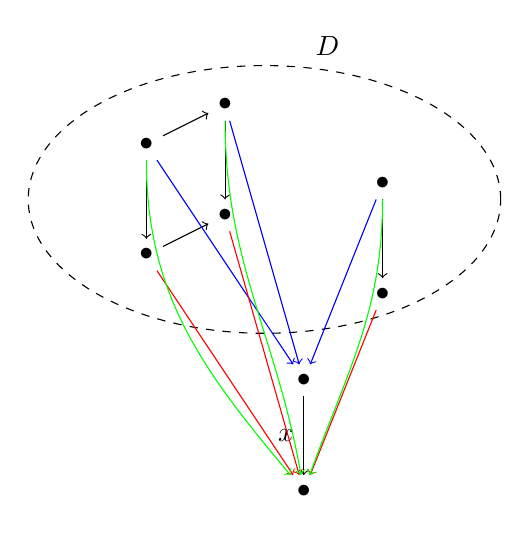
\begin{tikzpicture}
        \draw[->] (0,0)   node[above] (d1a) {$\bullet$}
              -- (0,-1)   node[below] (d1b) {$\bullet$};
        \draw[->] (1,.5)  node[above] (d2a) {$\bullet$}
              -- (1,-.5)  node[below] (d2b) {$\bullet$};
        \draw[->] (3,-.5) node[above] (d3a) {$\bullet$}
              -- (3,-1.5) node[below] (d3b) {$\bullet$};
        \draw[->] (d1a) -- (d2a);
        \draw[->] (d1b) -- (d2b);
        \draw[dashed] (1.5,-0.5) ellipse (3 and 1.7);
        \draw (2.3,1.2) node[above] {$D$};

        \draw[->] (2,-3) node[above] (xa) {$\bullet$}
              -- node[left] {$x$} (2,-4)  node[below] (xb) {$\bullet$};
        \draw[->,blue]  (d1a) -- (xa);
        \draw[->,blue]  (d2a) -- (xa);
        \draw[->,blue]  (d3a) -- (xa);
        \draw[->,red]   (d1b) -- (xb);
        \draw[->,red]   (d2b) -- (xb);
        \draw[->,red]   (d3b) -- (xb);
        \draw[->,green] (d1a) edge[out=270, in=130] (xb);
        \draw[->,green] (d2a) edge[out=270, in=100] (xb);
        \draw[->,green] (d3a) edge[out=270, in=70]  (xb);
    \end{tikzpicture}\end{center}

    Les flèches bleues indiquent des flèches dans l'image de $\arf$ et les flèches
    rouges sont dans l'image de $\id_{\C_\Sigma}$. Pour montrer que l'on a un cocône,
    il faut montrer que les carrés verticaux sont commutatifs, ce qui est immédiat
    puisque la flèche de $x$ vient de la propriétés de colimite de
    $\arf(\colim_I U_1\circ f)$ appliqué au cocône formé par les flèches vertes.

    On prends maintenant un cocône $c$ sur $D$. En composant par $U_1$ et $U_2$ on obtient
    qu'il existe au plus une flèche de $x$ vers $c$. Pour vérifier qu'il en existe une,
    il faut montrer qu'on peut obtenir un carré commutatif à partir des flèches de
    colimites dans $\cf$ et $\C_\Sigma$, ce qui est direct.
\end{pv}

\begin{cor}
    $U_1$ et $U_2$ sont exacts à droite.
\end{cor}

Afin de donner une description plus intéressante de quelques colimites usuelles, on
va définir une description en terme de séquent de objets de $\tsigma$.

\begin{defi}{Représentation en séquents de $\tsigma$}
    Soit $f : n\ast\rightarrow X$ un objet de $\tsigma$. On note
    $<\phi_X> = \Xi\vdash\Phi$. $f$ induit une fonction de $x_1,\dots x_n$ vers $\Xi$.
    On note le séquent associé à $f$ de la façon suivante~:

    \[ <f> := x_1, \dots x_n; \Xi - \im f\vdash \Phi',\mathcal{E} \]

    Où $\Phi'$ est $\Phi$ où l'on a remplacé chaque variable par une de ses préimage
    par $f$ si elle est dans l'image de $f$. De plus, $\mathcal{E}$ est une suite
    d'égalités~: $x_i=x_j\in\mathcal{E}$ si $f(x_i) = f(x_j)$ et $i\neq j$.

    Une formule de la forme $\Xi;\Gamma\vdash \Phi$ représente une formule ayant comme
    variables libre $\Xi$ et comme variables liées $\Gamma$. De plus on a toujours
    $\Xi\cap\Gamma=\emptyset$.
\end{defi}

\begin{exs}
    \item $<\iota\ast> = x;\vdash$
    \item $<\iota yR> = x_1,\dots x_{\ar(R)};\vdash R(x_1, \dots, x_{\ar(R)})$
    \item Si on note $\tilde{0} : 2\rightarrow 2$ la fonction constante égale à
        zéro, on peut prendre $\theta : 2\ast\rightarrow X$ où $X$ est une formule
        vide à deux variables telle que $\theta_\star = \tilde{0}$. Dans ce cas, on
        a $<\theta> = x,y;\vdash x = y$~: c'est la diagonale ! On remarque donc
        qu'avec ces conventions, il est possible de définir la diagonale même en
        l'absence de relation. Cela revient à dire que l'égalité fait toujours
        parti des relations autorisées, ce qui est une convention commune.
\end{exs}

\begin{lem}
    Soient $X,Y\in\tsigma$. On note $X+Y$ leur coproduit. Notons aussi
    $<X> = \Xi;\Gamma\vdash\Phi$ et $<Y> = \Xi';\Gamma'\vdash\Phi'$ (on suppose
    tous les ensembles de variables disjoints).
    
    Alors $<X+Y> = \Xi,\Xi';\Gamma,\Gamma'\vdash\Phi,\Phi'$.
\end{lem}

\begin{lem}
    Notons $\mathbf{0}$ l'élément initial de $\tsigma$.
    
    Alors $<\mathbf{0}> = ;\vdash$.
\end{lem}

\begin{lem}
    Soient $X,Y\in\tsigma$. On note $<X> = \Xi,x;\Gamma\vdash\Phi$ et
    $<Y> = \Xi',y;\Gamma'\vdash\Phi'$. On considère de plus les flèches allant de
    $<Z> = x;\vdash$ vers $X$ (resp $Y$) qui sélectionnent la variable $x$ (resp $y$).

    Alors $<X +_Z Y> = \Xi,\Xi',x;\Gamma,\Gamma'\vdash\Phi,\Phi'[y/x]$.
\end{lem}

\begin{pv}
    Tous ces lemmes sont des conséquences directes du théorème \ref{commaCL}.
\end{pv}

\begin{theo}{Relèvement sur $\tsigma$}\label{lifting}
    Soit $r : \C_\Sigma\rightarrow\tgamma$ un foncteur exact à droite. Alors il
    existe un foncteur exact à droite $\tilde{r}$ tel que~:

    \[\begin{tikzcd}
        \C_\Sigma\arrow[dr, bend right, "\iota"]\arrow[rr, bend left, "r"]
            & \cong & \tgamma \\
        & \tsigma\arrow[ur, bend right, "\tilde{r}"] & \\
    \end{tikzcd}\]
\end{theo}

\begin{pv}
    On commence par construire un $\tilde{r}$ candidat, puis on
    vérifiera qu'il est bien exact à droite.
    
    Soit $k\ast\xrightarrow{f} X\in\tsigma$. On note $r\ast = n\ast\rightarrow\phi$
    et $rX = m\ast\rightarrow\psi$. L'objet de $\tsigma$ étant une flèche de $\C_\Sigma$,
    elle est envoyée sur un carré commutatif. De plus, comme $r$ est exact à droite,
    on a $r(k\ast) = kr(\ast)$. Donc $r$ nous donne le carré commutatif suivant~:

    \[\begin{tikzcd}
        kn\ast\arrow[r, "r_1f"]\arrow[d]\arrow[dr,dashed] & m\ast\arrow[d] \\
        k\phi\arrow[r, "r_2f"] & \psi \\
    \end{tikzcd}\]

    On définit l'image de $f$ par $\tilde{r}$ comme étant la diagonale de ce carré
    commutatif. On doit maintenant définir l'image d'une flèche. Soit un carré commutatif
    dans $\tsigma$~:

    \[\begin{tikzcd}
        k_1\ast\arrow[r,"g_1"]\arrow[d,"f_1"] & k_2\ast\arrow[d,"f_2"] \\
        X_1\arrow[r,"g_2"] & X_2 \\
    \end{tikzcd}\]

    Comme l'image de chaque morphisme est un carré commutatif, donc en prenant
    l'image par $r$ on obtient la pyramide suivante~:

    \[\begin{tikzcd}
        k_1n\ast\arrow[rrr,red,"r_1g_1"]\arrow[dr]\arrow[ddd, "r_1f_1"]\arrow[ddr,dashed]
            & & & k_2n\ast\arrow[dl]\arrow[ddd, "r_1f_2"]\arrow[ddl,dashed] \\
        & k_1\phi\arrow[r,"r_2g_1"]\arrow[d,"r_2f_1"]
            & k_2\phi\arrow[d,swap,"r_2f_2"] & \\
        & \psi_1\arrow[r,red,"r_2g_2"]
            & \psi_2 & \\
        n_1\ast\arrow[ur]\arrow[rrr,"r_1g_2"]
            & & & n_2\ast\arrow[ul] \\
    \end{tikzcd}\]

    Les flèches en rouge nous donnent l'image du carré commutatif.

    On obtient facilement que $\tilde{r}$ préserve l'identité et la composition
    (on recolle les pyramides selon leur côté commun). C'est donc bien un foncteur.

    Construisons maintenant une transformation naturelle entre $rX$ et
    $\tilde{r}\iota X$. On définit $\theta_X$ comme étant le carré commutatif
    suivant~:

    \[\begin{tikzcd}
        kn\ast\arrow[r, "r_1f"]\arrow[d] & m\ast\arrow[d] \\
        \psi\arrow[r, "\id"] & \psi \\
    \end{tikzcd}\]

    Or $f$ est une flèche de $\tsigma$ créée par $\iota$, elle est donc bijective. Comme
    les foncteurs préservent les isomorphismes, $r_1f$ est un isomorphisme. On a donc
    une transformation inversible, vérifions qu'elle est naturelle~:

    \[\begin{tikzcd}
        kn\ast\arrow[rrrr, "r_1f"]\arrow[dr, "n\arf(h_\star)"]\arrow[dddddrr]
            & & & & m\ast\arrow[dl, swap, "r_1h"]\arrow[dddddll] \\
        & k'n\ast\arrow[rr, "r_1f'"]\arrow[ddr]
            & & m'\ast\arrow[ddl] & \\
        & & & & \\
        & & \psi' & & \\
        & & & & \\
        & & \phi\arrow[uu, "r_2h"] & & \\
    \end{tikzcd}\]

    La base et le sommet commutent. De plus, le côté droit et celui du haut commutent.
    Donc donc les faces commutent~: $\theta$ est un isomorphisme naturel entre
    $\tilde{r}\circ\iota$ et $r$.

    Il est aussi direct de vérifier que $\tilde{r}$ est exact à droite.
    % TODO détailler ?
\end{pv}


